\subsection{Resoluci\'on}

Para nuestra heurística golosa comenzamos ordenando las aristas por peso de mayor a menor. Una vez obtenida la lista de aristas ordenadas por peso la iteramos escogiendo primero un nodo (arbitrariamente) de la arista más pesada y si la arista aun no se encuentra ubicada, se agrega a un nuevo conjunto siempre y cuando no hayamos sobrepasado la cantidad $k$ de conjuntos creados. En caso de que ya tengamos $k$ conjuntos o en caso de que hayamos terminado de recorrer las aristas se termina el ciclo.
Ahora verificamos si la cantidad de conjuntos creados es menor a $k$, en caso afirmativo habremos ubicado todos los nodos con aristas en alguno de los conjuntos.
Si quedan nodos sin ubicar, estos se agregan a cualquier conjunto, como ya agregamos todos los nodos de grado mayor a uno, los que restan se puede decir que tienen grado 0, por lo tanto, no importa en que conjunto sean agregados, estos no crearán aristas intraparticion y como consecuencia no sumarán peso a ningún conjunto.
Si la cantidad de conjuntos creados es igual a $k$, actuamos de forma diferente, aquí recorremos todas las aristas, actuando solo con las que no hayan sido agregadas a ningún conjunto de la siguiente manera: verificamos cuanto peso agregaría en cada conjunto para luego realmente añadirlo al conjunto que sume menos peso, en caso de encontrar uno en el que no cree aristas intraparticion, es agregado a este sin seguir revisando los restantes.

Como se puede observar usamos dos componentes greedys en la heurística:
La primera esta cuando se ordenan las aritas decrecientemente y se crean los $k$ conjuntos a medida que se separan los nodos de las aristas de mayor peso, para que estos no generen aristas intraparticion.
La segunda componente greedy se encuentra cuando al finalizar de crear los $k$ conjuntos se recorre nodo por nodo verificando si ya se encuentra agregado y en caso negativo, verificando en que conjunto genera menos peso para finalmente agregarlo a este.

A modo de ejemplo presentamos algunas imagenes para mostrar el funcionamiento de la heuristica:

\begin{figure}[H]
\begin{center}
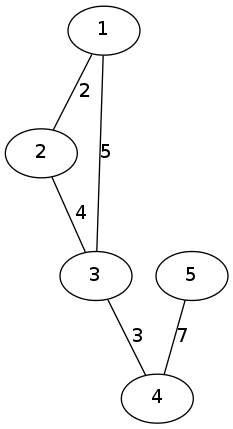
\includegraphics[scale=0.4]{./img/greedy1.png}
\caption{(1) Grafo de ejemplo}
\end{center}
\end{figure}
La primer imagen corresponde al grafo al que se le aplicará k-PMP (1)

\begin{figure}[H]
\begin{center}
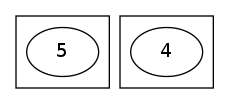
\includegraphics[scale=0.4]{./img/greedy2.png}
\caption{(2) Conjuntos 1 y 2 luego de separar los nodos de las aristas mas pesadas}
\end{center}
\end{figure}
Luego de ordenar las aristas escoge las de mayor tamaño y separa sus nodos en k conjuntos k=2 para este ejemplo. (2)

\begin{figure}[H]
\begin{center}
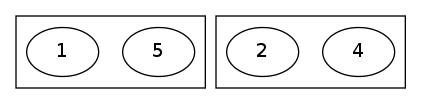
\includegraphics[scale=0.4]{./img/greedy3.png}
\caption{(3) Conjuntos luego de comenzar a ingresar los nodos restantes}
\end{center}
\end{figure}
Luego como ya hay 2 conjuntos creados procede a verificar nodo los nodos y agregandolos al conjunto que menos sume. En el caso del nodo 1, se agrega de inmediato al primer conjunto porque no genera arista intraparticion. Para el nodo 2 primero verifica en el 1er conjunto, aqui sumaria 2 de peso, se verifica en el siguiente conjunto, y como no suma peso, se ingresa ahí. (3)

\begin{figure}[H]
\begin{center}
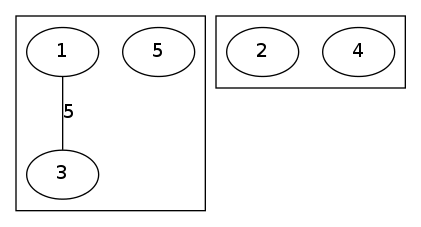
\includegraphics[scale=0.4]{./img/greedy4.png}
\caption{(4) Resultado de haber corrido la heuristica greedy al grafo (1)}
\end{center}
\end{figure}
Finalmente resta agregar el nodo 3 el cual genera en el conjunto uno un peso igual a 5, y en el conjunto 2 un peso igual a 7 al unirse con los nodos 2 y 4. Por lo tanto el nodo 3 es introducido en el conjunto 1. (4)


A continuación presentamos un pseudo-grafico del algoritmo
\begin{itemize}
\item ordenar $aristas$ por peso en orden decreciente
\item mientras restan $aristas$ 
  \begin{itemize}
  \item si no hay $k$ conjuntos, crear conjunto y agregar $nodo1$ de $arista$ (si este no pertenece a ningún conjunto)
  \item sino cortar el ciclo  
  \item si no hay $k$ conjuntos, crear conjunto y agregar $nodo2$ de $arista$ (si este no pertenece a ningún conjunto)
  \item sino cortar el ciclo  
  \end{itemize}
\item Si hay menos de $k$ conjuntos creados
  \begin{itemize}
  \item agregar las aristas que quedaron fuera a alguno de los conjuntos creados
  \end{itemize}
\item Sino
  \begin{itemize}
  \item desde nodo 0 a nodo n-1
    \begin{itemize}
    \item si el nodo no esta en ningún conjunto
      \begin{itemize}
        \item verificar conjunto por conjunto cuanto peso generaría agregarlo a este
        \item agregar el nodo al conjunto en el que genere menos peso
      \end{itemize}
    \end{itemize}
  \end{itemize}
\end{itemize}




\subsection{Analisis de complejidad}

Vamos a analizar el codigo paso por paso analizando la complejidad temporal del peor caso.
Lo primero que hacemos es ordernar las aristas, para esto utilizamos la funcion $sort$ de la $std$ que posee una complegidad temporal de $O(n.log(n))$, en este caso como se aplica a las aristas esto es $O(m.log(m))$ siendo $m$ la cantidad de aristas.
A continuación, y haciendo uso del psudo-codigo proporcionado:
\begin{itemize}
\item mientras restan $aristas$ 
  \begin{itemize}
  \item si no hay $k$ conjuntos, crear conjunto y agregar $nodo1$ de $arista$ (si este no pertenece a ningún conjunto)
  \item sino cortar el ciclo  
  \item si no hay $k$ conjuntos, crear conjunto y agregar $nodo2$ de $arista$ (si este no pertenece a ningún conjunto)
  \item sino cortar el ciclo  
  \end{itemize}
\end{itemize}
Este scope tiene una complejidad $O(m)$ ya que se recorren todas las aritas, en el peor caso creando conjuntos y agregandolos a estos, pero estas dos acciones tienen una complejidad constante.

A continuacion si se crearon menos de $k$ conjuntos se agregan los nodos que restan a uno de estos. En el peor caso esto pertenece al orden de $O(n)$ siendo n la cantidad de nodos.
Si hay $k$ conjuntos creados se procede de la siguiente manera:
\begin{itemize}
\item desde nodo 0 a nodo n-1   $O(n)$
  \begin{itemize}
  \item si el nodo no esta en ningún conjunto $O(1)$
    \begin{itemize}
      \item verificar conjunto por conjunto cuanto peso generaría agregarlo a este $O(k+n)$
      \item agregar el nodo al conjunto en el que genere menos peso $O(1)$
    \end{itemize}
  \end{itemize}
\end{itemize}

Esta ultima parte del algoritmo tiene una complejidad acotada en el peor caso de O(n^2) ya que por cada nodo no agregado ($n$ en total en el peor caso) se verifica cuanto pesaría agregarlo a cada conjunto. Para esto se recorren los nodos ya ingresados en el conjunto actual (peor caso $n$) y se agrega al que menor peso aporte. Esto tiene relacion con el $k$ tambien ya que en el peor caso se verificará en los $k$ conjuntos.

\subsection{Instancias desfavorables}


Probamos la heuristica con varias familias de grafos, grafos estrella...(ETC) 
Para el caso de los grafos estrella nuestra heuristica funcionaba mal, particularmente cuando el numero del nodo central era superior a la cantidad k de conjuntos. 
Para aclarar, en un principio nuestro algoritmo constaba solo de la segunda componente greedy de la que se habla en la seccion Resolucion. Por lo que comenzaba desde el primer nodo hasta el ultimo probando en que conjunto convenia poner dicho nodo de forma de disminuir lo mas posible el peso total de las aristas intraparticion. Volviendo al caso del grafo estrella, lo que pasaba era que ingresaba en los

\subsection{Experimentacion}

Para poder observar la performance del algoritmo en terminos de tiempo de ejecucion en funcion al tamaño de la entrada nos contruimos un script en python que genera tres tipos de grafos, grafos con un 15 porciento de aristas, uno con un 50 porciento de aristas y el último con el 100 porciento de aristas, tomando para el porcentaje la cantidad de aristas que llevaria un grafo completo.
Para cada uno de estos variamos los valores de n y de k con n entre 100 y 500. 
Por cada uno de esos valores de n, variamos el valor de k entre 2 y 10.
Cada una de todas estas instancias fueron corridas entre 20 y 30 veces, (20 para las instancias mas grandes) para poder calcular un promedio. Ya que consideramos que el procesador no esta ejecutando solo nuestra heurística, por lo que el tiempo que le toma correr el algoritmo hasta obtener una solucion seguramente es mayor al real. Por otro lado tambien pensamos en la posibilidad de que el procesador cachee las soluciones al estar haciendo muchas veces lo mismo, razon por la cual decidimos no superar las 30 repeticiones. Entre estas dos cosas donde una desfavorece y otra favorece el tiempo de ejecucion, nos parecio razonable realizar un promedio.
Con los valores obtenidos presentamos algunos graficos para tener una descripcion mas visual y los analizamos.

\begin{figure}[H]
\begin{center}
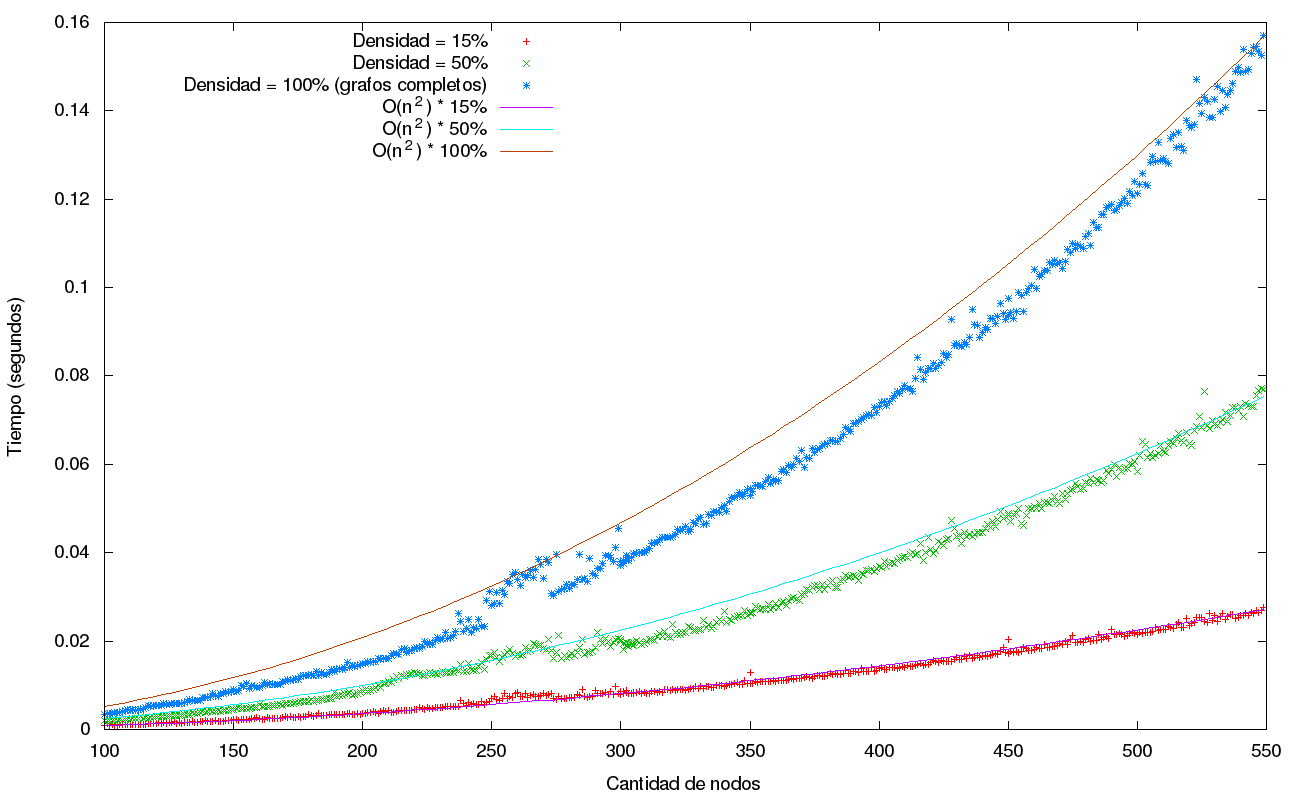
\includegraphics[scale=0.4]{./img/greedyN1.png}
\caption{Graficos de}
\end{center}
\end{figure}

\begin{figure}[H]
\begin{center}
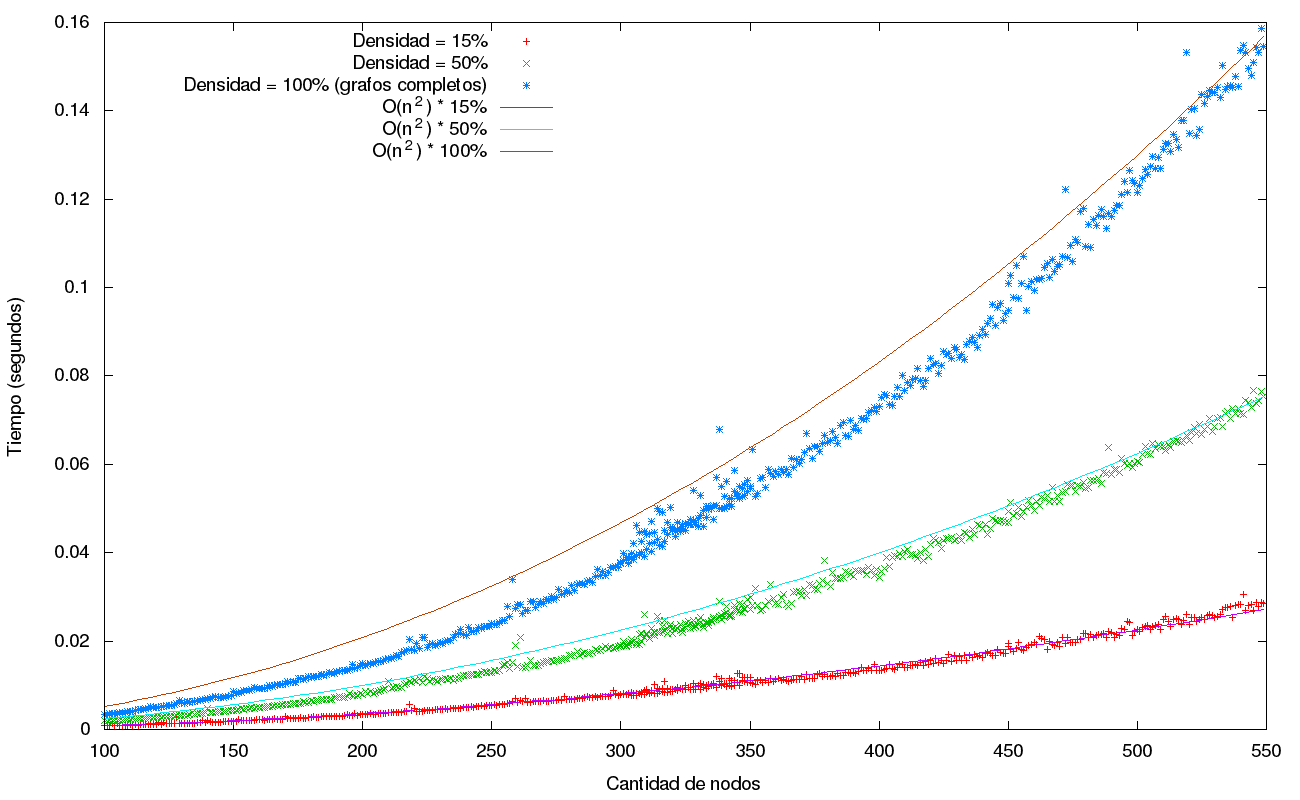
\includegraphics[scale=0.4]{./img/greedyN2.png}
\caption{Graficos de}
\end{center}
\end{figure}

\begin{figure}[H]
\begin{center}
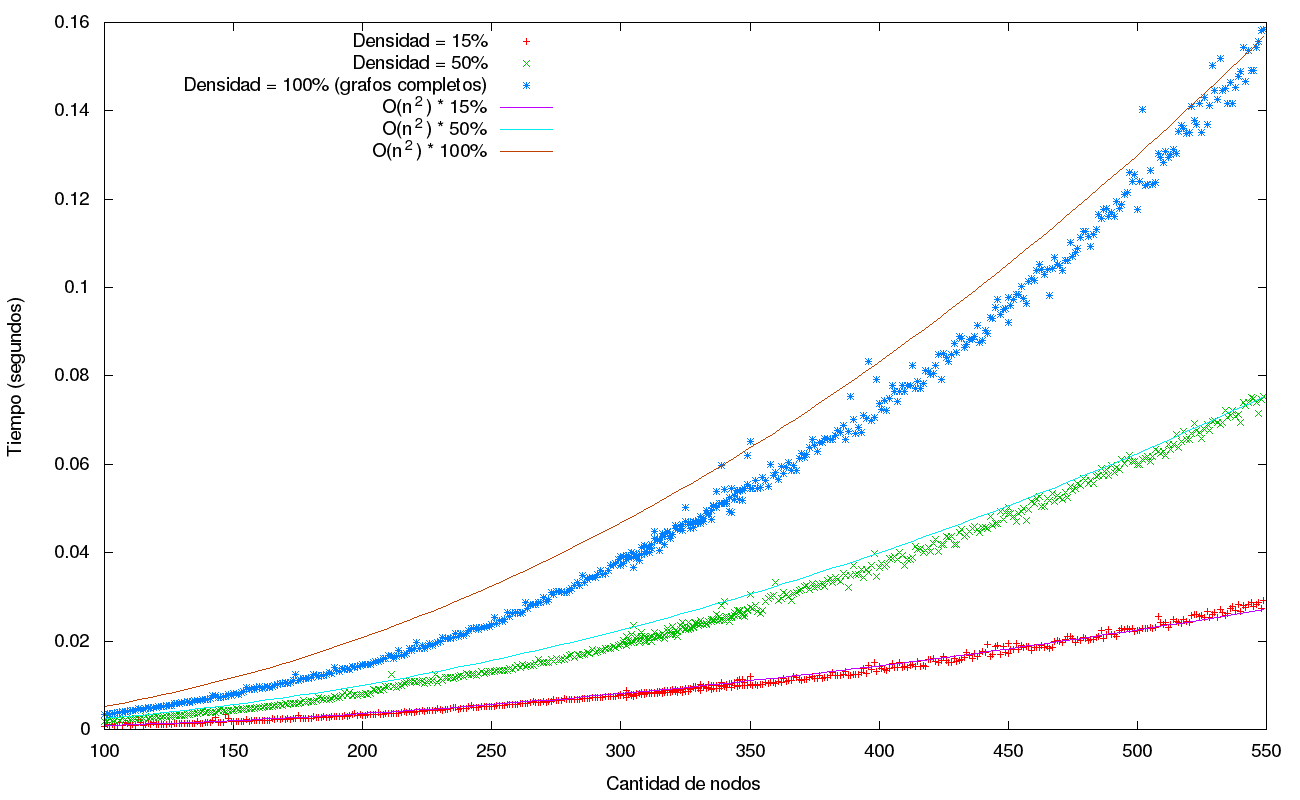
\includegraphics[scale=0.4]{./img/greedyN3.png}
\caption{Graficos de}
\end{center}
\end{figure}


En estos graficos podemos observar que el algoritmo tiene una complejidad de n^2 en relacion a la cantidad de nodos, la cual obviamente se ve afectada al mismo tiempo por la cantidad de aristas que el grafo posee. Esta observacion se puede notar ya que cada grafo presenta la complejidad temporal para una densidad de aristas de 15\%, 50\% y 100\% comparada con un valor n^2 multiplicado por una constante obtenida a partir de dividir el tiempo sobre la cantidad de nodos, y a su vez este valor es multiplicado por 0.15, 0.50 y 1.
Al hacer esto y verificar que los valores se asemejan demasiado podemos concluir que la cantidad de aristas del grafo afecta directamente al rendimiento de forma lineal.

En los tres graficos utilizamos los mismos valores para O(n^2)* densidad de cantidad de aristas, y como se puede observar comparando los distintos graficos, que presentan una variacion en la cantidad k de conjuntos, los valores resultantes de los tests son casi los mismos, no se nota ninguna variacion apreciable. 



%\begin{figure}[H]
%\begin{center}
%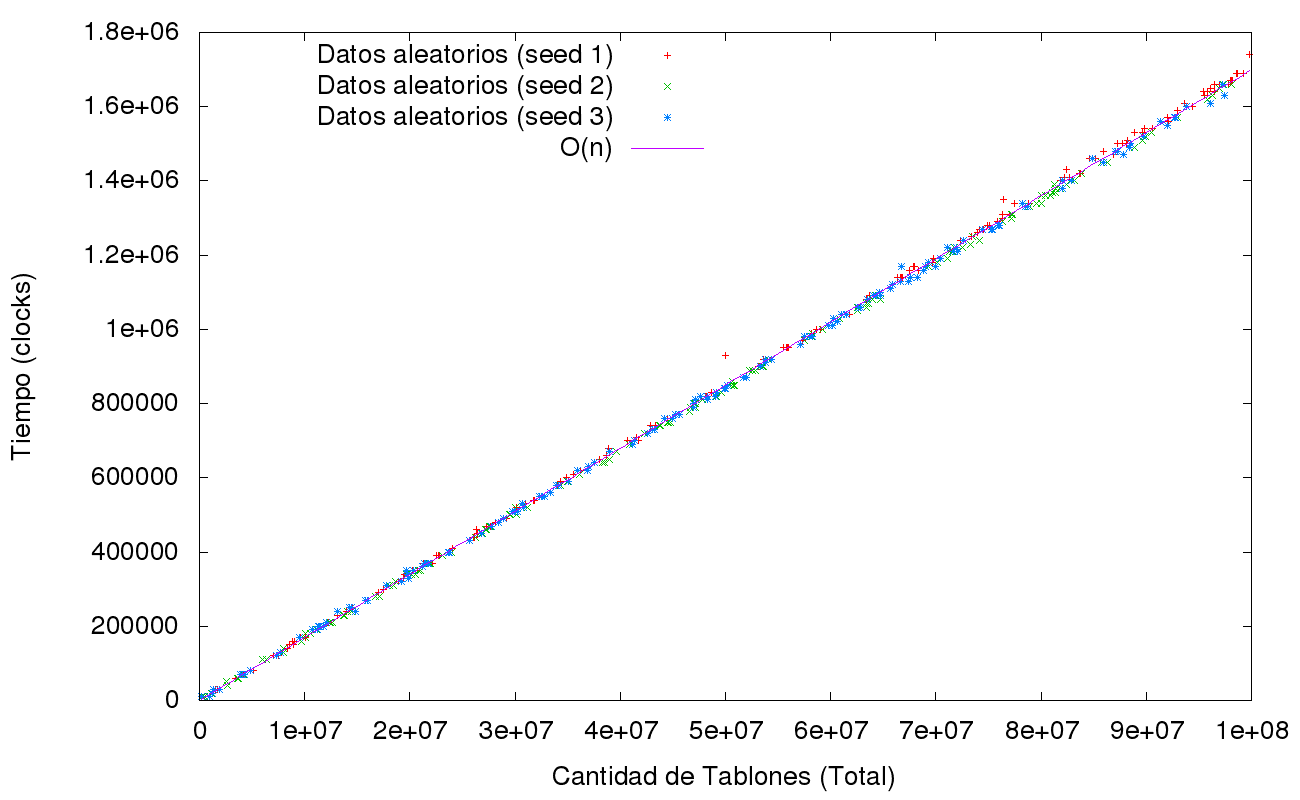
\includegraphics[scale=0.4]{./imagenes/ej1_chartRendimiento.png}
%\caption{Gr\'afico de tiempos con test pseudo-aleatorios.}
%\end{center}
%end{figure}

